\pdfoutput=1
\documentclass[a4paper,pdftex,10pt]{article}
% \usepackage[whole,autotilde]{bxcjkjatype}
\usepackage[T1]{fontenc}
\usepackage{tgtermes}

% ---Display \subsubsection at the Index
\setcounter{tocdepth}{3}

% ---Setting about the geometry of the document----
\usepackage{a4wide}
% \pagestyle{empty}

% ---Physics and Math Packages---
\usepackage{amssymb,amsfonts,amsthm,mathtools}
\usepackage{physics,braket,bm,slashed}

% ---underline---
\usepackage[normalem]{ulem}

% ---cancel---
\usepackage{cancel}

% --- surround the texts or equations
\usepackage{fancybox,ascmac}

% ---settings of theorem environment---
\theoremstyle{definition}
\newtheorem{dfn}{Definition}
\newtheorem{prop}{Proposition}
\newtheorem{thm}{Theorem}

% ---settings of proof environment---
\renewcommand{\proofname}{\textbf{Proof}}
\renewcommand{\qedsymbol}{$\blacksquare$}

% ---Ignore the Warnings---
\usepackage{silence}
\WarningFilter{latexfont}{Some font shapes,Font shape}
\ExplSyntaxOn
\msg_redirect_name:nnn{hooks}{generic-deprecated}{none}
\ExplSyntaxOff

% ---Insert the figure (If insert the `draft' at the option, the process becomes faster.)---
% \usepackage{graphicx}
% \usepackage{subcaption}

% ----Add a link to a text---
\usepackage{url,hyperref}
\usepackage[dvipsnames,svgnames]{xcolor}
\hypersetup{colorlinks=true,citecolor=FireBrick,linkcolor=Navy,urlcolor=purple}

% ---Tikz---
\usepackage{tikz,pgf,pgfplots,circuitikz}
\pgfplotsset{compat=1.15}
\usetikzlibrary{intersections, arrows.meta, angles, calc, 3d, decorations.pathmorphing}
\usepackage[compat=1.1.0]{tikz-feynhand}

% ---tcolorbox---
\usepackage{tcolorbox}
\tcbuselibrary{raster,skins,breakable}
\newtcolorbox{graybox}[1][]{frame empty, colback=black!07!white, sharp corners}

% ---Add the section number to the equation, figure, and table number---
\makeatletter
   \renewcommand{\theequation}{$\thesection.\arabic{equation}$}
   \@addtoreset{equation}{section}
   
   \renewcommand{\thefigure}{\thesection.\arabic{figure}}
   \@addtoreset{figure}{section}
   
   \renewcommand{\thetable}{\thesection.\arabic{table}}
   \@addtoreset{table}{section}
\makeatother

% ---enumerate---
% \renewcommand{\labelenumi}{$\arabic{enumi}.$}
% \renewcommand{\labelenumii}{$(\arabic{enumii})$}

% ---Index---
% \usepackage{makeidx}
% \makeindex 

% ---footnotes---
\renewcommand{\thefootnote}{$\ast$\arabic{footnote}}

% ---Title---
\title{Notes on Anomalies}
\author{Itsuki Miyane}
\date{Last modified:\ \today}

\begin{document}

\maketitle

\begin{enumerate}
  \item
        If we put $\theta=\pi/2$, the quantity $\Sigma$ becomes $r^2$ and the line element is obtained as
        \begin{equation}
          \dd s^2
          =
          -
          c^2
          \left( 1-\frac{2\mu}{r} \right)\dd t^2
          -
          \frac{4\mu ac}{r}\dd t\dd \varphi
          +
          \frac{r^2}{\Delta}\dd r^2
          +
          \left(
          r^2+a^2+\frac{2\mu a^2}{r}
          \right)
          \dd\varphi^2
        \end{equation}
        and the metric also is as
        \begin{equation}
          g_{\mu\nu}
          =
          \begin{pmatrix}
            -c^2(1-2\mu/r) & 0          & -2\mu ac/r            \\
            0              & r^2/\Delta & 0                     \\
            -2\mu ac/r     & 0          & r^2 + a^2 +2\mu a^2/r
          \end{pmatrix}
        \end{equation}
        where $\Delta$ still remain $r^2-2\mu r+a^2$. We obtain its inverse
        \begin{equation}
          g^{\mu\nu}
          =
          \begin{pmatrix}
            -\dfrac{r^3+a^2(r+2\mu)}{c^2 r(a^2+r^2-2\mu r)} & 0                          & -\dfrac{2a\mu}{a^2 cr+cr^3-2cr^2\mu} \\
            0                                               & \dfrac{a^2+r^2-2r\mu}{r^2} & 0                                    \\
            -\dfrac{2a\mu}{a^2cr+cr^3-2cr^2\mu}             & 0                          & \dfrac{r-2\mu}{a^2+r^3-2r^2\mu}
          \end{pmatrix}
          \label{eqn:inverse_metric}
        \end{equation}
        and $\dot{t}$ and $\dot{\varphi}$ are, then, immediately derived as
        \begin{graybox}
          \vspace*{-12pt}
          \begin{align}
            \dot{t}
             & =
            g^{tt}p_{t}+g^{t\varphi}p_{\varphi}
            \nonumber
            \\
             & =
            \dfrac{ckr^3-2ah\mu+a^2 ck(r+2\mu)}{cr(a^2+r(r-2\mu))}
            ,
            \\
            \dot{\varphi}
             & =
            g^{\varphi t}p_{t}+g^{\varphi\varphi}p_{\varphi}
            \nonumber
            \\
             & =
            \dfrac{hr-2h\mu+2ack\mu}{a^2r+r^3-2r^2\mu}
            .
          \end{align}
        \end{graybox}


  \item

        What we need to do is just insert the inverse metric which we already obtained \eqref{eqn:inverse_metric} into
        \begin{align}
          g^{\mu\nu}p_{\mu}p_{\nu}
           & =
          g^{tt}p_{t}^2
          +
          g^{\varphi\varphi}p_{\varphi}^2
          +
          2g^{t\varphi}p_{t}p_{\varphi}
          +
          g^{rr}p_{r}^2
          \nonumber
          \\
           & =
          g^{tt}\cdot(-kc^2)^2
          +
          g^{\varphi\varphi}\cdot h^2
          +
          2g^{t\varphi}\cdot(-kc^2)\cdot h
          +
          g_{rr}\dot{r}^2
          .
        \end{align}
        Note that we use the fact that $p_{r}$ is obtained by lowering the indices $\dot{r}$, i.e. $p_{r}=g_{rr}\dot{r}$. Putting the inverse matrix components $g^{\mu\nu}$ and organizing the equations, we will get the effective potential as
        \begin{graybox}
          \begin{equation}
            V_{\mathrm{eff}}(r)
            =
            \frac{h^2-a^2c^2(k^2-1)}{2r^2}
            -
            \frac{(h-ack)^2\mu}{r^3}
            -
            \frac{c^2\mu}{r}
            .
          \end{equation}
        \end{graybox}
        It is obvious that $V_{\mathrm{eff}}(r)$ satisfies the relation
        \begin{equation}
          \frac{1}{2}\dot{r}^2
          +
          V_{\mathrm{eff}}(r)
          =
          \frac{1}{2}c^2(k^2-1)
        \end{equation}
        obtained from $g^{\mu\nu}p_{\mu}p_{\nu}=-c^2$ since it was defined to satisfy that equation.


  \item
        Since we will analyze the circular motion, we can put $\dot{r}$ to zero in the previous result. Therefore the last result becomes
        \begin{equation}
          \frac{h^2-a^2c^2(k^2-1)}{2}u^2
          -
          x^2\mu u^3
          -
          c^2\mu u
          =
          \frac{1}{2}c^2(k^2-1)
          \label{eqn:relation1}
        \end{equation}
        and solving to $x^2$, we find
        \begin{equation}
          x^2
          =
          \frac{1}{2\mu u^3}c^2(k^2-1)
          +
          \frac{c^2}{u^2}
          +
          \frac{1}{2\mu u}\left[ h^2-a^2c^2(k^2-1) \right]
          .
        \end{equation}
        We still use $x^2$ when we derive $k$ and $h$ and insert the solution
        \begin{equation}
          x
          =
          -
          \sqrt{
            \frac{1}{2\mu u^3}c^2(k^2-1)
            +
            \frac{c^2}{u^2}
            +
            \frac{1}{2\mu u}\left[ h^2-a^2c^2(k^2-1) \right]
          }
          (<
          0)
          \label{eqn:x}
        \end{equation}
        to the obtained expression at the final step. To evaluate two values $k$ and $h$, we should prepare one more relation for $k$ and $h$. Since we are assuming the circular motion, its orbits should be stabilized at the potential minimum. So, to express such a situation, we will consider the extremum condition\footnote{
          It is obvious that the extremum condition for $V_{\textrm{eff}}$ does not depend on the variables $r, u$. It means that
          $$
            \dv{V_{\textrm{eff}}}{r}
            =
            0
            \ \iff\
            \dv{V_{\textrm{eff}}}{u}
            =
            0
            .
          $$
        }
        \begin{equation}
          \dv{V_{\textrm{eff}}}{u}
          =
          \left\{ h^2-a^2c^2(k^2-1) \right\}u
          -
          3x^2\mu u^2
          -
          c^2\mu
          =
          0
          \label{eqn:relation2}
        \end{equation}
        and solve \eqref{eqn:relation2} with \eqref{eqn:relation1} to $k$ and $h$. Then we finally obtain
        \begin{graybox}
          \vspace*{-5pt}
          \begin{gather}
            k
            =
            -\frac{\sqrt{c^2 (1-\mu  u)+\mu  u^3 x}}{c}
            \label{eqn:k}
            \\
            h
            =
            -
            \sqrt{\dfrac{\mu  \left(c^2 \left(1-a^2 u^2\right)+u^2 x \left(a^2 \
                u^2+3\right)\right)}{u}}
            \label{eqn:h}
          \end{gather}
          with $x$ in \eqref{eqn:x}.
        \end{graybox}
        
        Note that $x$ remains in the result. I regard $x$ as a constant since I guess so from the problem statement.  


  \item
        To evaluate the innermost stable circular orbit, we should derive a second-order derivative
        \begin{equation}
          \dv[2]{V_{\textrm{eff}}}{r}
          =
          \frac{3 \left(h^2-a^2 c^2 \left(k^2-1\right)\right)}{r^4}-\frac{12\mu(h-a c k)^2}{r^5}-\frac{2 c^2 \mu }{r^3}
        \end{equation}
        and take it to zero. This equality decides the orbit radius $r$. To make coefficients just depend on $\mu$ and $a$, we should vanish $k$ and $h$ by using the previous result. Thus, inserting the last results \eqref{eqn:k}, \eqref{eqn:h} and \eqref{eqn:x} and organizing messy expression, we can find the equality for $r$ as
        \begin{graybox}
          \vspace*{-12pt}
          \begin{equation}
            \mu  r^2 \left(r (r-6 \mu ) (r-3 \mu )-a^2 (7 \mu +3 r)\right)-6 \sqrt{\mu ^3 r^3 \left(a^3+a r (r-2 \mu )\right)^2}
            =
            0
            .
          \end{equation}
        \end{graybox}

\end{enumerate}

\begin{figure}
  \centering
  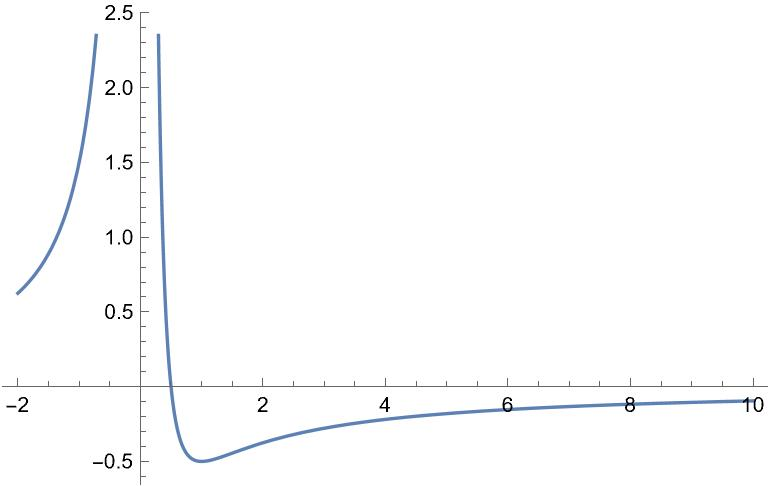
\includegraphics[width=0.8\textwidth]{fig/Veff.jpg}
  \caption{One example of the effective potential $V_{\textrm{eff}}$}
\end{figure}


% ----------------------------------------------------------------------
\begin{thebibliography}{99}
  \bibitem{url01}
  \href{https://www.roma1.infn.it/teongrav/onde19_20/geodetiche_Kerr.pdf}{Chapter 22 Geodesic motion in Kerr spacetime}. (Last accessed: \today)
  \bibitem{url02}
  \href{https://www.pas.rochester.edu/assets/pdf/undergraduate/kerr_geometry_and_rotating_black_holes.pdf}{Kerr Geometry and Rotating Black Hole}. (Last accessed: \today)
\end{thebibliography}

% ----------------------------------------
% \appendix
% \section{The computation of the radius of the photon sphere}











% ----------------------------------------
% \clearpage
% \bibliography{ref}
% \bibliographystyle{ytamsalpha}

% ----------------------------------------
% \clearpage
% \index{hoge@hoge}
% \printindex

\end{document}
